\section{Mott insulators}\label{sec:mott}

Band theory was found to be flawed soon after it was introduced. The picture it proposes is simple and generally works pretty well. It is based on considering the electrons to be independently moving under the constant background potential created by the ions. The solutions of the Schr\"odinger for free electrons in a periodic potential $U(\bm r)$, such that $U(\bm r) = U(\bm r + \bm R)$,

\begin{equation}\label{eq:schrodinger}
\bigg[ -\frac{1}{2m} \nabla^2 + U(\bm r) \bigg] \psi (\bm r) = \varepsilon \psi (\bm r)
\end{equation}
are given by Bloch's theorem: $\psi_{\bm k} (\bm r) = e^{i\bm k \cdot \bm r} u_{\bm k} (\bm r)$. Note that we made $\hbar = 1$. Replacing this wave function in equation (\ref{eq:schrodinger}), we obtain a differential equation for $u_{\bm k} (\bm r)$, which has in general an infinite number of solutions. We label them with an index $n$, which we call the band index. To each solution there corresponds a function $\varepsilon_{n\bm k}$. The set of these functions is known as the band structure. Since electrons are taken to be independent in band theory, the N-electron eigenstates are obtained by placing an electron in each quantum state. Each state is labelled by its energy $\varepsilon_{n\bm k \sigma}$. Since our model Hamiltonian does not couple spins (via an electron interaction, for example) and assuming there is no external magnetic field and that the system has an inversion center, we have $\varepsilon_{n\bm k \uparrow} = \varepsilon_{n\bm k \downarrow}$. In general there might be energies for which there is no corresponding $\varepsilon_{n\bm k \sigma}$. These form intervals called forbidden bands\footnote{We disregard surface states that may have energies that fall in the forbidden bands.}. Thus, the ground state of our model may be obtained by filling the energy levels starting from the lowest energy state. Two cases are particularly relevant:
\begin{itemize}
\item Every band is either fully occupied or empty. The first excited state differs from the ground state by $\Delta$, the separation between the last fully occupied band and the first empty band. It is then impossible to induce the motion of the electrons by applying an arbitrarily small voltage. This is what it means to be an \emph{insulator}. Since there $2N$ states per band, this is not possible unless the number of electrons per unit cell is an even integer.
\item One or more of the bands are partially filled. The energy of occupied state of higher energy is named the Fermi energy $\varepsilon_F$. In this case, the separation between the ground state and the first excited state tends to $0$ in the thermodynamic limit, $N \rightarrow \infty$. The system may then respond to infinitesimal excitations, which is the  definition of a metal.
\end{itemize}

Band theory made it possible to predict whether a solid would be a metal or an insulator. However, its success rests crucially on the independent electron approximation. Thus, it is not surprising that for compounds with strongly correlated electrons the theory might fail \cite{Mila2007}. The Coulomb interaction is in general non negligible, and the effects it leads to are not captured by a mean field approach. One must resort to many-body theory. An example of a many-body effect that band theory doesn't capture is (conventional) superconductivity. However, this does not deem band theory useless. In fact, the superconducting phase arises due to an instability of a state that is itself well described by band theory \cite{deGennes1999}. A far greater failure of band theory is that predicts certain compounds with an odd number of electrons per unit cell, such as \chem{NiO} and \chem{La_2 Cu O_4},  to be metals, while in fact  they turn out to be (Mott) insulators. Mott devised a simple argument to justify this failure. It is based on considering the elementary electronic excitations of a solid composed by hydrogen atoms as a function of the distance between atoms.

Consider a hypothetical solid consisting of a square lattice with hydrogen atoms on its points. Each unit cell has one hydrogen atom, and consequently one electron. Band theory would predict such a solid to be a metal. However, if the lattice parameter $a$ is large enough, the solid cannot remain a metal. There must be some value of the lattice parameter $a = a_c$ for which the system becomes an insulator. When current flows through a sample of this solid, electrons hop consecutively, reaching positions that can be quite far on the lattice. For a metal, this process occurs even when exciting the system with an infinitesimal amount of energy. How much energy do we need to provide for this process to occur?

\begin{figure}[ht!]\label{hubbardOneHoleOneDoublyOc}
\centering
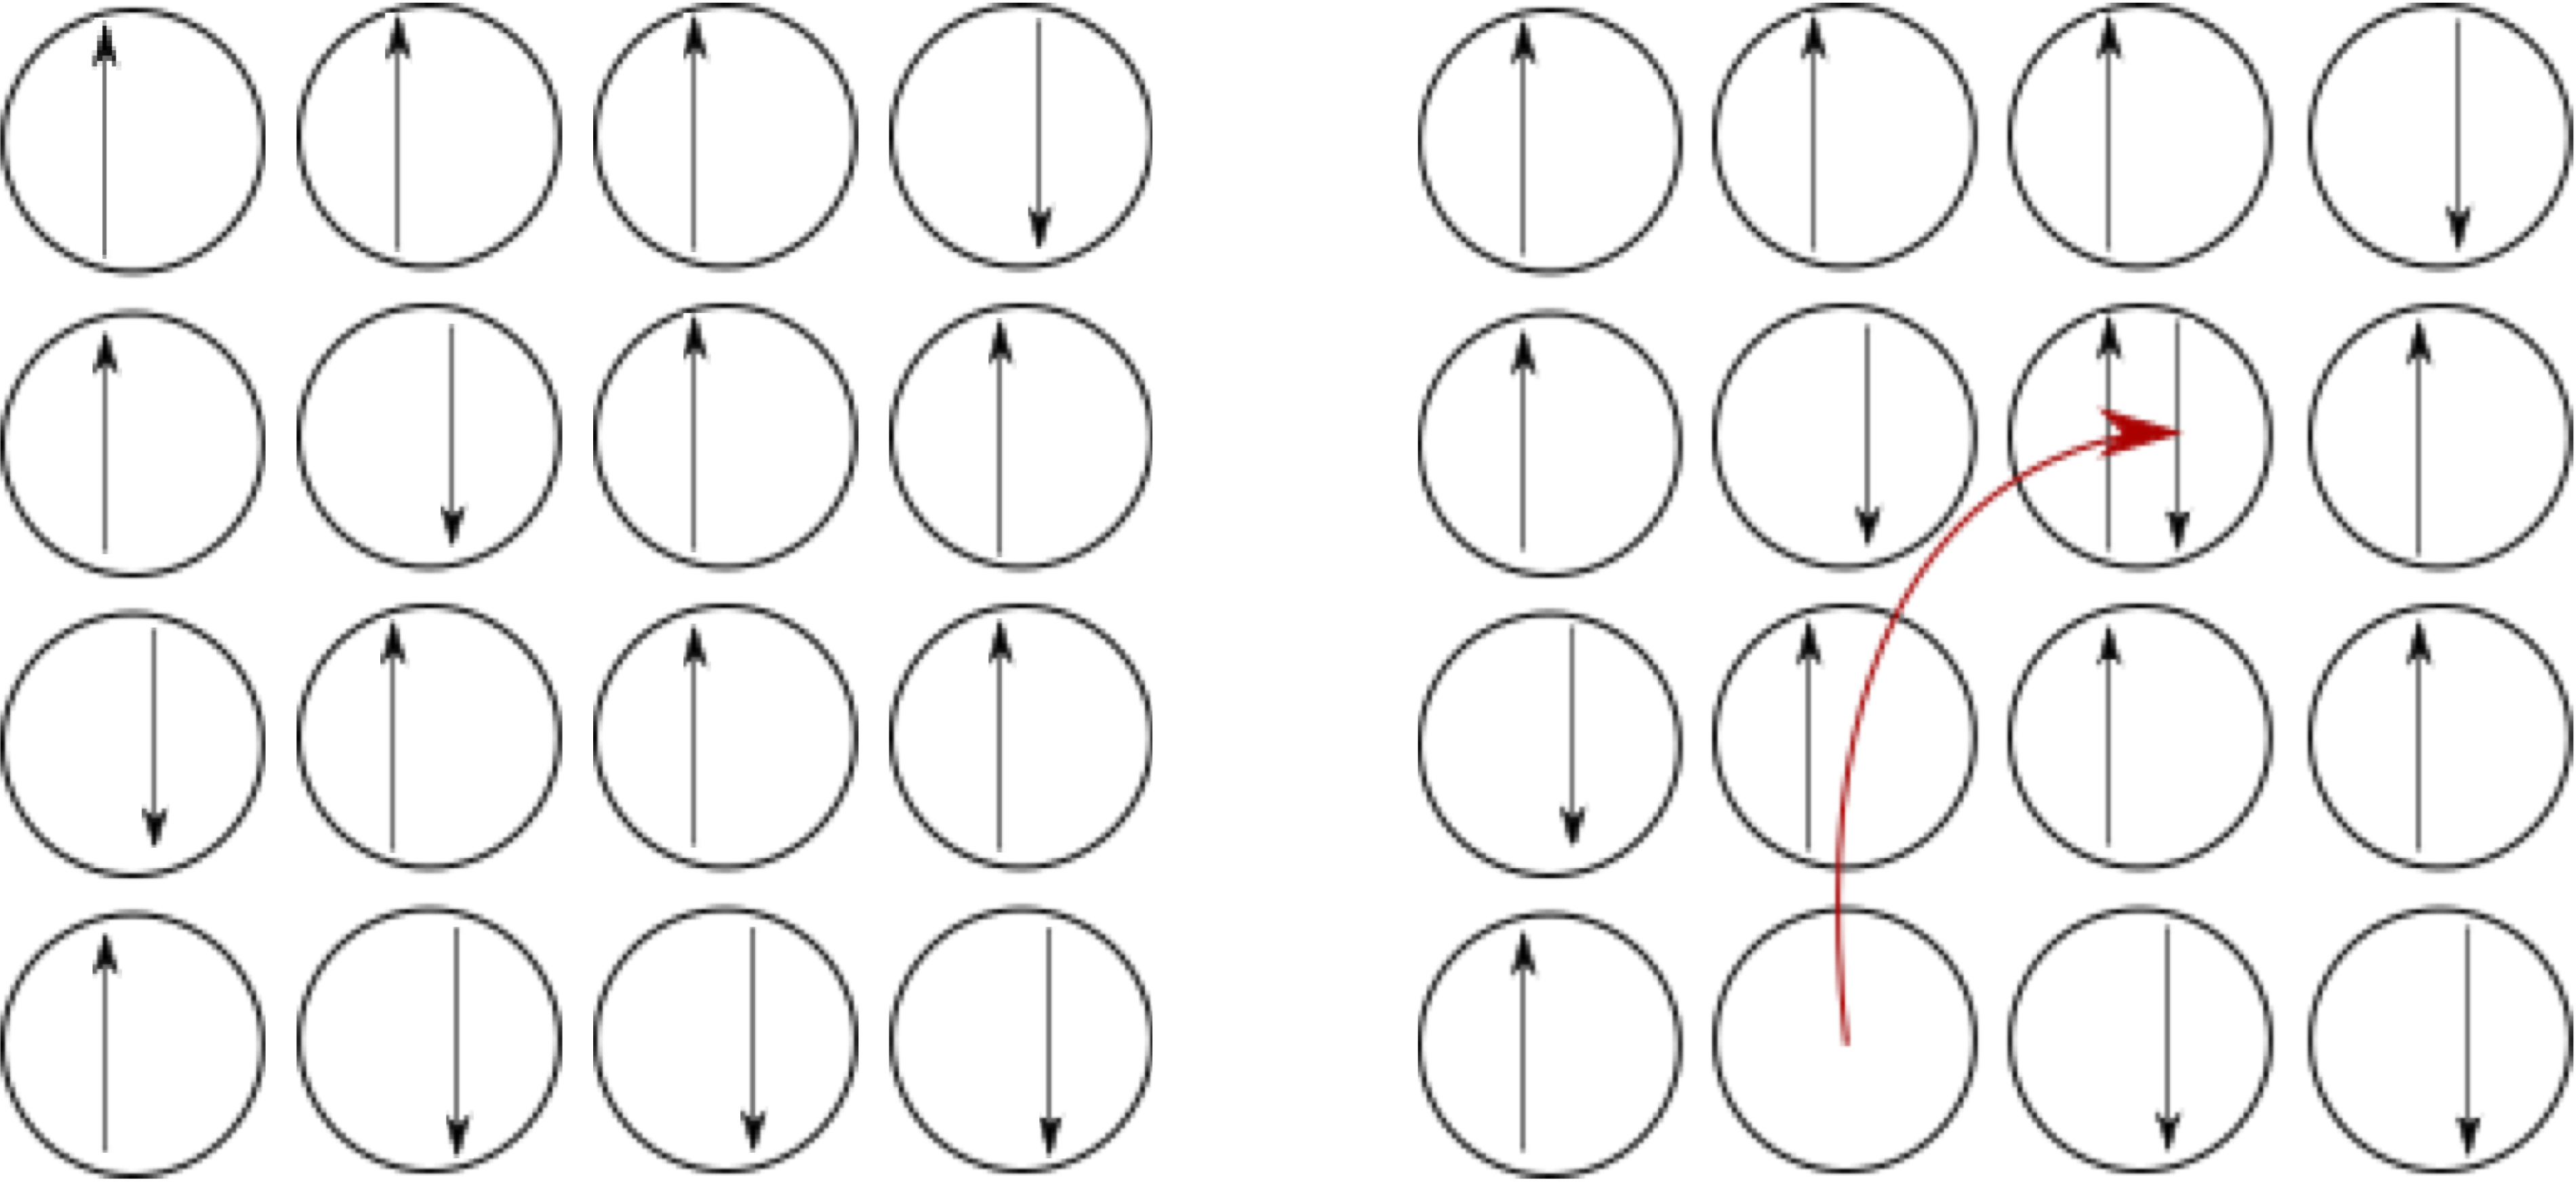
\includegraphics[width = 9cm]{Figures/HubbardModel/hubbardOneHoleOneDoublyOcV2.png}
\caption[Configuration of the Hubbard model on the square lattice with a hole and a doubly occupied site.]{On the right, a configuration on the square lattice with a hole and a doubly occupied site obtained by delocalization of the spin down electron on the left.}
\end{figure}

If $a$ is large, we have essentially one electron per site at the start. When an electron is displaced, we end up with a hole and a doubly occupied site. The potential energy of such a state is

\begin{equation}
E_{H^-} + E_{H^+} - 2 E_H 
\end{equation}

Due to the Coulomb repulsion between the two electrons in $H^-$, this quantity is strictly positive. Call it $U > 0$. On the other hand, the system also has kinetic energy: both the hole and the doubly occupied site can delocalize. Let $W$ be the bandwidth corresponding to the delocalization of an electron on the lattice. Both the hole and the doubly occupied will stay at the bottom of the band and gain an energy $W/2$ (assuming that this delocalization is of the same order of magnitude). The dominant transfer integral $-t$ is between nearest neighbors. The dispersion relation then reads

\begin{equation}
\varepsilon_{\bm k} = -2 t ( \cos k_x + \cos k_y ) 
\end{equation}

The bandwidth is then $W = 8 t$. The energy of a configuration with a hole and a doubly occupied site is

\begin{equation}
\Delta_c = U - W ,
\end{equation}
where $U$ is practically independent of the lattice parameter $a$. The bandwidth $W$, however, depends strongly on $a$. When $a \gg a_0$, where $a_0$ is the Bohr radius, the transfer integral is exponentially small, because only the exponential tails of the wave functions are relevant. In this limit, $\Delta_c \approx U$ is a large, positive number, and the system is an insulator. This type of insulator is called a Mott insulator, and $\Delta_c$ is called the charge gap. As $a$ decreases, $t$ increases, and there must be a critical value $a_c \sim a_0$, for which $U = W$. Below this value, the computation of $\Delta_c$ is not valid anymore because the gap cannot be negative. Thus, there must be a metal-insulator transition. It is possible to see this transition if we apply enough pressure to a Mott insulator so as to decrease $a$ and increase $t$. A transition of this type was first seen in the 1970's for $V_2 O_3$\footnote{Of course, the transition is not so easy to describe. However, this simple argument provides an intuitive picture.}. There is a fundamental difference between a band insulator and a Mott insulator. While we must pay an energy $\Delta_c$ to make a charge excitation, this is not the cost of a spin excitation: we can flip the spin of an electron without creating a doubly occupied site. The fluctuations of both charge and spin due to the electron interactions may then lead to magnetic behavior characteristic of this type of systems.